\documentclass[12pt]{beamer}
\usepackage{listings}
\usepackage[]{color}
%\usepackage{bbding}
%\usepackage{ragged2e}
%\usepackage{tikz}
%\usetikzlibrary{decorations.pathreplacing}

\beamertemplatenavigationsymbolsempty
\AtBeginSection[]
{
    \begin{frame}
    \frametitle{Table of Contents}
    \tableofcontents[currentsection]
    \end{frame}
}
\setlength{\tabcolsep}{10pt}
\newcommand{\bigoh}[1]{\ensuremath{\mathcal{O}\left(#1\right)}}
\newcommand{\TLE}{\textcolor{blue}{TLE}}
\newcommand{\WA}{\textcolor{red}{WA}}
\newcommand{\MLE}{\textcolor{orange}{MLE}}
\newcommand{\AC}{\textcolor{green}{AC}}
\newcommand{\blank}{\vspace{.5cm}}

\definecolor{mygreen}{rgb}{0,0.6,0}
\definecolor{mygray}{rgb}{0.5,0.5,0.5}
\definecolor{mymauve}{rgb}{0.58,0,0.82}

\iffalse
\lstset{ %
  backgroundcolor=\color{white},   % choose the background color; you must add \usepackage{color} or \usepackage{xcolor}
  basicstyle=\tiny,        % the size of the fonts that are used for the code
  breakatwhitespace=false,         % sets if automatic breaks should only happen at whitespace
  breaklines=true,                 % sets automatic line breaking
  commentstyle=\color{mygreen},    % comment style
  deletekeywords={...},            % if you want to delete keywords from the given language
  escapeinside={\%*}{*)},          % if you want to add LaTeX within your code
  extendedchars=true,              % lets you use non-ASCII characters; for 8-bits encodings only, does not work with UTF-8
  frame=single,                    % adds a frame around the code
  keepspaces=true,                 % keeps spaces in text, useful for keeping indentation of code (possibly needs columns=flexible)
  keywordstyle=\color{blue},       % keyword style
  language=C++,                 % the language of the code
  morekeywords={*,...},            % if you want to add more keywords to the set
  numbers=left,                    % where to put the line-numbers; possible values are (none, left, right)
  numbersep=5pt,                   % how far the line-numbers are from the code
  numberstyle=\tiny\color{mygray}, % the style that is used for the line-numbers
  rulecolor=\color{black},         % if not set, the frame-color may be changed on line-breaks within not-black text (e.g. comments (green here))
  showspaces=false,                % show spaces everywhere adding particular underscores; it overrides 'showstringspaces'
  showstringspaces=false,          % underline spaces within strings only
  showtabs=false,                  % show tabs within strings adding particular underscores
  stepnumber=1,                    % the step between two line-numbers. If it's 1, each line will be numbered
  stringstyle=\color{mymauve},     % string literal style
  tabsize=2                      % sets default tabsize to 2 spaces
}
\fi

\title{Fenwick Tree}
\subtitle{Binary Indexing, Least Significant One-bit}
\author{beOI Training}
\institute{
\includegraphics[height=12em]{../share/beoi-logo}}

\begin{document}

\frame{\titlepage}

\section{Motivation}

\begin{frame}
    \frametitle{Motivating Problem}
    Dynamic Range Sum Query \\\blank
    Well, can't we simply use a Segment Tree?  \\\blank
    Yes we can, but the Fenwick Tree datastructure has some cool advantages.
\end{frame}

\section{How it works}

\begin{frame}
    \frametitle{How it works}
    Let's define $rsq(i)$ as the sum of the elements from $1$ up to $i$
    \[ rsq(i) = A[1] + A[2] + \cdots + A[i] \]
    We can then answer any range sum query by computing
    \[ rsq(a, b) = rsq(b) - rsq(a-1) \]
    We also need a point update function $update(k, v)$
    which updates element $k$ to a new value $v$. \\\blank
    Like segment trees, Fenwick trees address these functions in
    $\bigoh{\log n}$.
\end{frame}

\begin{frame}
    \frametitle{Least Significant One-bit}
    The \textbf{least significant 1-bit} of an integer is the rightmost 1-bit
    of its \textbf{binary representation}. \\
    \begin{align*}
        (42)_{10} &= (1010\textcolor{red}{1}0)_2 \\
        (1337)_{10} &= (1010011100\textcolor{red}{1})_2 \\
        (2016)_{10} &= (11111\textcolor{red}{1}00000)_2
    \end{align*}
    Let's define function $LSOne(i)$ as the least significant 1-bit isolated
    from $i$
    \begin{align*}
        LSOne(42) &= 0000\textcolor{red}{1}0 \\
        LSOne(1337) &= 0000000000\textcolor{red}{1} \\
        LSOne(2016) &= 0000\textcolor{red}{1}00000
    \end{align*}
\end{frame}

\begin{frame}
    \frametitle{Binary Indexing}
    Like in segment trees, each node is responsible for
    (i.e. stores the sum of) a certain range of elements. \\\blank
    Specifically, node $i$ is responsible for range
    \[ [ i - LSOne(i) + 1;  i ] \]
    This range has size $LSOne(i)$. \\\blank
    e.g. $LSOne(2016) = 32$, thus node $2016$ will store sum of range
    $[1985; 2016]$ which has size $32$.
\end{frame}

\begin{frame}
    \frametitle{Visualization}
    \begin{center}
        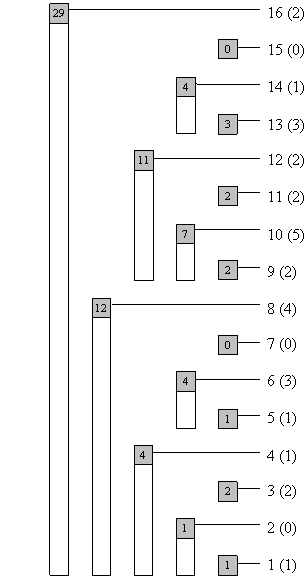
\includegraphics[width=\linewidth,height=.8\textheight,keepaspectratio]{img/tree}
    \end{center}
\end{frame}

\begin{frame}
    \frametitle{Querying}
    One can observe that
    \begin{alignat*}{4}
        & rsq(13) &&= ft[1101] &&+ ft[1100] &&+ ft[1000] \\
        & &&= rsq(13, 13) &&+ rsq(9, 12) &&+ rsq(1, 8)
    \end{alignat*}
    So to obtain $rsq(i)$ we need to iteratively strip off $LSOne(i)$ and sum
    the values stored at the nodes we come accross.
\end{frame}

\begin{frame}
    \frametitle{Query Visualization}
    \begin{center}
        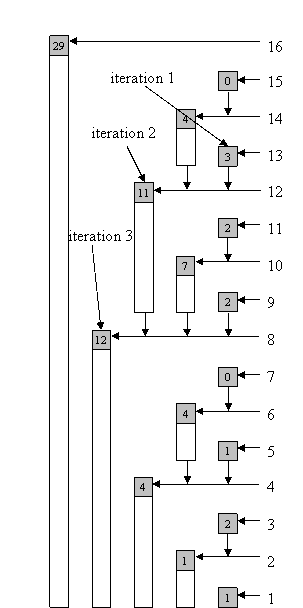
\includegraphics[width=\linewidth,height=.8\textheight,keepaspectratio]{img/query}
    \end{center}
\end{frame}

\begin{frame}
    \frametitle{Query Complexity}
    The number of iterations is equal to the number of 1-bits in the starting
    index. \\\blank
    If the starting index $n$ consists of $b$ bits, we need at most $b$
    operations to find $rsq(n)$.
    \[ \bigoh{b} = \bigoh{\log n} \]
\end{frame}

\begin{frame}
    \frametitle{LSOne Implementation}
    There is a binary trick to compute the Least Significant One-bit
    really fast
    \[ LSOne(i) = (i\ \&\ (-i)) \]
\end{frame}

\begin{frame}
    \frametitle{Query Implementation}
    \lstinputlisting{src/ft-query.cpp}
\end{frame}

\begin{frame}
    \frametitle{Updating}
    When updating index $i$, we need to update all nodes that are responsible
    for index $i$. \\\blank
    Specifically, if we update index $i$ from $v_\mathrm{old}$ to 
    $v_\mathrm{new}$, we need to add 
    $v_\mathrm{new} - v_\mathrm{old}$ to each node responsible for index $i$.
\end{frame}

\begin{frame}
    \frametitle{Updating}
    One can prove that if node $k$ is responsible for index $i$, then
    node $k + LSOne(k)$ is the smallest node $>k$ that is also responsible
    for $i$.

    \begin{align*}
        38 &= (1001\textcolor{red}{1}0)_2 \\
        38 + LSOne(38) = 40 &= (101000)_2
    \end{align*}
\end{frame}

\begin{frame}
    \frametitle{Updating}
    $i$ is the smallest node responsible for index $i$. \\\blank
    Thus, to find all nodes responsible for $i$, we can simply start from $i$
    and iteratively add the Least Significant 1-bit. \\\blank
    \begin{align*}
        \text{update } (10\textcolor{red}{1})_2 &= 5 \\
        \text{update } (1\textcolor{red}{1}0)_2 &= 6 \\
        \text{update } (\textcolor{red}{1}000)_2 &= 8 \\
        \text{update } (\textcolor{red}{1}0000)_2 &= 16 \\
        &\vdots
    \end{align*}
    When do we stop? When we arrive at a node outside our initial array.
\end{frame}

\begin{frame}
    \frametitle{Update Visualization}
    \begin{center}
        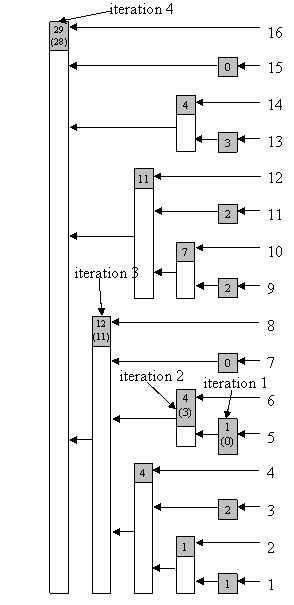
\includegraphics[width=\linewidth,height=.8\textheight,keepaspectratio]{img/update}
    \end{center}
\end{frame}

\begin{frame}
    \frametitle{Update Complexity}
    When adding $LSOne(i)$, the least significant bit is shifted at least
    1 place to the left. \\\blank
    So, in the worst case, we need to loop through all bits until we get to an
    index $>n$.
    \[ \bigoh{\log n} \]
\end{frame}

\begin{frame}
    \frametitle{Update Implementation}
    \lstinputlisting{src/ft-update.cpp}
\end{frame}

\begin{frame}
    \frametitle{Building}
    To build the Fenwick Tree from the array $A$, there is no better way than
    updating each index separately.
    \[ \bigoh{n\log n} \]
\end{frame}

\section{Segment Tree vs Fenwick Tree}

\begin{frame}
    \frametitle{Time Complexity}
    \begin{center}
        \begin{tabular}{c|c|c}
            & Segment Tree & Fenwick Tree \\
            \hline
            Query & \bigoh{\log n} & \bigoh{\log n} \\
            Update & \bigoh{\log n} & \bigoh{\log n} \\
            Build & \bigoh{n} & \bigoh{n \log n} 
        \end{tabular}
    \end{center}
    In general, Fenwick Trees are slightly more efficient because of the fast
    bit trick and few memory accesses.
\end{frame}

\begin{frame}
    \frametitle{Memory Usage}
    Both use \bigoh{n} memory.
\end{frame}

\begin{frame}
    \frametitle{Code}
    Segment Tree: ~40 lines of code \\\blank
    Fenwick Tree: ~10 lines of code! \\\blank
    In contest, always use Fenwick if possible!
\end{frame}

\begin{frame}
    \frametitle{Applications}
    Beware: you cannot use Fenwick Trees for any function of your liking.
    \[ rsq(a, b) = rsq(b) - rsq(a-1) \]
    There is \textbf{no} such property for min/max, so Fenwick is not suitable
    for Dynamic RMQ.
\end{frame}

\end{document}
